\documentclass[12pt,a4paper]{article}

%Russian-specific packages
%--------------------------------------
\usepackage[T2A]{fontenc}
\usepackage[utf8]{inputenc}
\usepackage[russian]{babel}
%--------------------------------------

\setlength\parindent{0pt} %% Do not touch this

\usepackage{geometry}
 \geometry{
 a4paper,
 total={170mm,257mm},
 left=20mm,
 top=20mm,
 }

\usepackage{blkarray}
\usepackage{amsmath}
\usepackage{mathtools}
\usepackage{enumitem}
\usepackage{graphicx}
\graphicspath{{./images/}}
\usepackage{tikz}
\usepackage{tikz-network}
\usetikzlibrary{tikzmark}
\usepackage{wrapfig}
\usepackage{caption}
\usepackage{colortbl}
\usepackage{amssymb}
\usepackage{eqparbox}
\usepackage{outlines}

\usepackage[normalem]{ulem}
\newcommand{\stkout}[1]{\ifmmode\text{\sout{\ensuremath{#1}}}\else\sout{#1}\fi}

\usepackage{tocloft}
\renewcommand{\cftsecleader}{\cftdotfill{\cftdotsep}}
% \usepackage{biblatex}

% rome numbers
\makeatletter
\newcommand*{\rom}[1]{\expandafter\@slowromancap\romannumeral #1@}
\makeatother

\setcounter{MaxMatrixCols}{15}

%% -----------------------------
%% TITLE
%% -----------------------------
% \title{Курсовая работа по теории графов.} %% Assignment Title

% \author{Артём Черница\\ %% Student name
% группа М8О-104Б-19\\ %% Code and course name
% \textsc{Московский Авиационный Институт\\}
% \textsc{Вариант 22}
% }

% \date{\today} %% Change "\today" by another date manually
%% -----------------------------
%% -----------------------------

%% %%%%%%%%%%%%%%%%%%%%%%%%%
\begin{document}
%% %%%%%%%%%%%%%%%%%%%%%%%%%
% \maketitle
\addcontentsline{toc}{section}{Титульный лист}
\begin{titlepage}
   \begin{center}

      \textsc{МОСКОВСКИЙ АВИАЦИОННЫЙ ИНСТИТУТ \\
      (НАЦИОНАЛЬНЫЙ ИССЛЕДОВАТЕЛЬСКИЙ УНИВЕРСИТЕТ) \\
      ФАКУЛЬТЕТ ИНФОРМАЦИОННЫХ ТЕХНОЛОГИЙ И ПРИКЛАДНОЙ МАТЕМАТИКИ \\
      КАФЕДРА МАТЕМАТИЧЕСКОЙ КИБЕРНЕТИКИ}

      \vspace*{\fill}
      \textsc{\textbf{\Huge{КУРСОВАЯ РАБОТА}}\\
      \large{РАСКРАСКА ВЕРШИН ГИПЕРГРАФА}
      }
      \vspace*{\fill}

      \vfill
      \begin{flushright}
         \begin{minipage}{2.5in}
            \large{ 
               Студент: Черница А.А. \\
               Группа: М8О-104Б-19 \\ 
               Преподаватель: Яшина Н.П. \\
               Оценка: \\
               Дата: \\
            }
         \end{minipage}
      \end{flushright}
      
   \end{center}
\end{titlepage}

% --------------------------
% Start here
% --------------------------

\setcounter{page}{2}
% %%%%%%%%%%%%%%%%%%%
\section*{Задание}
\addcontentsline{toc}{section}{Задание}
% %%%%%%%%%%%%%%%%%%%
\paragraph*{1. Определить для орграфа заданного матрицей смежности:}
   \[
      A = \begin{pmatrix}
         0 & 1 & 1 & 1 \\
         0 & 0 & 1 & 0 \\
         0 & 1 & 0 & 0 \\
         1 & 1 & 1 & 0
      \end{pmatrix}
   \]
   Определить:
   \begin{enumerate}[label=(\alph*)]
      \item Матрицу односторонней связности.
      \item Матрицу сильной связности.
      \item Компоненты сильной связности.
      \item Матрицу контуров.
   \end{enumerate}

\paragraph*{2. Используя алгоритм Терри, определить замкнутый маршрут, проходящий ровно по два раза (по одному в каждом направлении) через каждое ребро графа.}
\begin{center}
   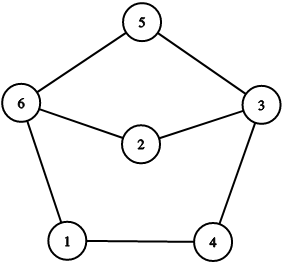
\includegraphics[scale=0.5]{terry.png}
\end{center}

\paragraph*{3. Используя алгоритм «фронта волны», найти все минимальные пути из первой вершину в последнюю орграфа, заданного матрицей смежности.}
   \[
      A = \begin{pmatrix}
         0 & 0 & 0 & 0 & 1 & 1 & 0 \\
         1 & 0 & 1 & 0 & 1 & 1 & 0 \\
         1 & 1 & 0 & 1 & 1 & 0 & 0 \\
         0 & 0 & 1 & 0 & 1 & 1 & 1 \\
         1 & 1 & 0 & 0 & 0 & 1 & 0 \\
         0 & 0 & 1 & 0 & 1 & 0 & 0 \\
         1 & 1 & 0 & 1 & 1 & 0 & 0
      \end{pmatrix}
   \]

\paragraph*{4. Используя алгоритм Форда, найти минимальные пути из первой вершины во все достижимые вершины в нагруженном графе, заданном матрицей длин дуг.}
      \[
         C = \begin{pmatrix}
            \infty & 2 & 7 & 8 & \infty & \infty & \infty \\
            12 & \infty & 4 & \infty & 6 & \infty & \infty \\
            \infty & 4 & \infty & 1 & 3 & 5 & 7 \\
            \infty & \infty & 1 & \infty & \infty & 3 & \infty \\
            \infty & \infty & 3 & \infty & \infty & \infty & 5 \\
            \infty & \infty & 5 & \infty & \infty & \infty & 2 \\
            2 & \infty & \infty & 3 & 4 & 6 & 7
         \end{pmatrix}
      \]

\paragraph*{5. Найти остовное дерево с минимальной суммой длин входящих в него рёбер.}
   \begin{center}
      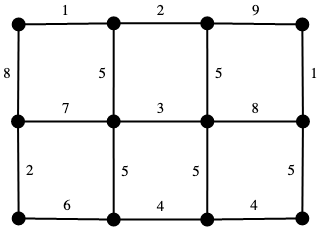
\includegraphics[scale=0.7]{spanning_tree.png}
   \end{center}

\paragraph*{6. Пусть каждому ребру неориентированного графа соответствует некоторый элемент электрической цепи. Составить линейно независимые системы уравнений Кирхгофа для токов и напряжений. Пусть первому и пятому ребру соответствуют источники тока с ЭДС E1 и E2, а остальные элементы являются сопротивлениями. Используя закон Ома, и, предполагая внутренние сопротивления источников тока равными нулю, получить систему уравнений для токов.}
   \begin{center}
      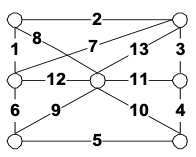
\includegraphics[scale=0.8]{kirhgof.png}
   \end{center}

\paragraph*{7. Построить максимальнй поток по транспортной сети.}
\begin{center}
   \begin{tikzpicture}[scale=1.5]
      %% vertices
      \draw[fill=black] (0,0) circle (3pt); % 1
      \draw[fill=black] (2,1) circle (3pt); % 2
      \draw[fill=black] (4,2) circle (3pt); % 3
      \draw[fill=black] (6,1) circle (3pt); % 4
      \draw[fill=black] (8,0) circle (3pt); % 5
      \draw[fill=black] (6,-1) circle (3pt); % 6
      \draw[fill=black] (4,-2) circle (3pt); % 7
      \draw[fill=black] (2,-1) circle (3pt); % 8
      \draw[fill=black] (4,0) circle (3pt); % 9

      %% vertex labels
      \node at (0,0.5) {v1};
      \node at (2,1.5) {v2};
      \node at (4,2.5) {v3};
      \node at (6,1.5) {v4};
      \node at (8,0.5) {v5};
      \node at (6,-1.5) {v6};
      \node at (4,-2.5) {v7};
      \node at (2,-1.5) {v8};
      \node at (4,0.5) {v9};

      %% edges
      % v1 -> v2
      \draw[thick,style={->,>=latex}] (0,0) -- (1.9,1) node [midway,fill=white] {\small{6}};
      
      % v2 -> v3
      \draw[thick,style={->,>=latex}] (2,1) -- (3.9,2) node [midway,fill=white] {\small{6}};
      
      % v3 -> v4
      \draw[thick,style={->,>=latex}] (4,2) -- (5.9,1) node [midway,fill=white] {\small{7}};
      
      % v4 -> v5
      \draw[thick,style={->,>=latex}] (6,1) -- (7.9,0) node [midway,fill=white] {\small{9}};
      
      % v6 -> v5
      \draw[thick,style={->,>=latex}] (6,-1) -- (7.9,0) node [midway,fill=white] {\small{16}};
      
      % v7 -> v6
      \draw[thick,style={->,>=latex}] (4,-2) -- (5.9,-1) node [midway,fill=white] {\small{9}};
      
      % v8 -> v7
      \draw[thick,style={->,>=latex}] (2,-1) -- (3.9,-2) node [midway,fill=white] {\small{3}};
      
      % v1 -> v8
      \draw[thick,style={->,>=latex}] (0,0) -- (1.9,-1) node [midway,fill=white] {\small{3}};
      
      % v1 -> v9
      \draw[thick,style={->,>=latex}] (0,0) -- (3.9,0) node [midway,fill=white] {\small{6}};
      
      % v9 -> v5
      \draw[thick,style={->,>=latex}] (4,0) -- (8,0) node [midway,fill=white] {\small{5}};
      
      % v1 -> v3
      \draw[thick,style={->,>=latex,bend right=30}] (0,0) to (3.9,2) node [below=10pt,sloped, fill=white] {8};
      
      % v1 -> v7
      \draw[thick,style={->,>=latex,bend left=30}] (0,0) to (3.9,-2) node [above=10pt,sloped, fill=white] {9};
      
      % v2 -> v9
      \draw[thick,style={->,>=latex}] (2,1) -- (3.9,0) node [midway,fill=white] {\small{2}};
      
      % v8 -> v9
      \draw[thick,style={->,>=latex}] (2,-1) -- (3.9,0) node [midway,fill=white] {\small{7}};
      
      % v9 -> v4
      \draw[thick,style={->,>=latex}] (4,0) -- (5.9,1) node [midway,fill=white] {\small{3}};
      
      % v9 -> v6
      \draw[thick,style={->,>=latex}] (4,0) -- (5.9,-1) node [midway,fill=white] {\small{6}};

   \end{tikzpicture}
\end{center}

\paragraph*{8. Раскраска вершин гиперграфа.}
% Лекции по теории графов/Емеличев В.А., Мельников О.И., Сарванов В.И., Тышкевич Р.И. -- М.: Наука, 1990 -- 384 с.
% Теория графов. Алгоритмический подход/Н.Кристофидес -- М.: Мир, 1978 -- 432 с.

\newpage

% %%%%%%%%%%%%%%%%%%%
\section*{Задание 1}
\addcontentsline{toc}{section}{Задание 1}
% %%%%%%%%%%%%%%%%%%%
   \textbf{a)} \rom{1} способ \\[10pt]
      $T = E \vee A \vee A^2 \vee A^3;$ \\[10pt]
      $
      A^2 = \begin{pmatrix}
         0 & 1 & 1 & 1 \\
         0 & 0 & 1 & 0 \\
         0 & 1 & 0 & 0 \\
         1 & 1 & 1 & 0
      \end{pmatrix} \cdot 
      \begin{pmatrix}
         0 & 1 & 1 & 1 \\
         0 & 0 & 1 & 0 \\
         0 & 1 & 0 & 0 \\
         1 & 1 & 1 & 0
      \end{pmatrix} = 
      \begin{pmatrix}
         1 & 1 & 1 & 0 \\
         0 & 1 & 0 & 0 \\
         0 & 0 & 1 & 0 \\
         0 & 1 & 1 & 1
      \end{pmatrix}
   $ \\[10pt]
   $
   A^3 = \begin{pmatrix}
      1 & 1 & 1 & 0 \\
      0 & 1 & 0 & 0 \\
      0 & 0 & 1 & 0 \\
      0 & 1 & 1 & 1
   \end{pmatrix} \cdot
   \begin{pmatrix}
      0 & 1 & 1 & 1 \\
      0 & 0 & 1 & 0 \\
      0 & 1 & 0 & 0 \\
      1 & 1 & 1 & 0
   \end{pmatrix} = 
   \begin{pmatrix}
      0 & 1 & 1 & 1 \\
      0 & 0 & 1 & 0 \\
      0 & 1 & 0 & 0 \\
      1 & 1 & 1 & 0
   \end{pmatrix}
   $ \\[10pt]
   $
   T = \begin{pmatrix}
      1 & 0 & 0 & 0 \\
      0 & 1 & 0 & 0 \\
      0 & 0 & 1 & 0 \\
      0 & 0 & 0 & 1
   \end{pmatrix} \vee
   \begin{pmatrix}
      0 & 1 & 1 & 1 \\
      0 & 0 & 1 & 0 \\
      0 & 1 & 0 & 0 \\
      1 & 1 & 1 & 0
   \end{pmatrix} \vee
   \begin{pmatrix}
      1 & 1 & 1 & 0 \\
      0 & 1 & 0 & 0 \\
      0 & 0 & 1 & 0 \\
      0 & 1 & 1 & 1
   \end{pmatrix} \vee
   \begin{pmatrix}
      0 & 1 & 1 & 1 \\
      0 & 0 & 1 & 0 \\
      0 & 1 & 0 & 0 \\
      1 & 1 & 1 & 0
   \end{pmatrix} = 
   \begin{pmatrix}
      1 & 1 & 1 & 1 \\
      0 & 1 & 1 & 0 \\
      0 & 1 & 1 & 0 \\
      1 & 1 & 1 & 1
   \end{pmatrix}
   $ \\[10pt]
   $T$ -- матрица односторонней связности. \\[10pt]
   \rom{2} cпособ \\[10pt]
   $T^{(n)} = t_{ij}^{(n)} = t_{ij}^{(n-1)} \vee (t_{in}^{(n-1)} \;\&\; t_{nj}^{(n-1)})$\\[10pt]
   $T^{(0)} = \begin{pmatrix}
      1 & 0 & 0 & 0 \\
      0 & 1 & 0 & 0 \\
      0 & 0 & 1 & 0 \\
      0 & 0 & 0 & 1  
   \end{pmatrix} \vee
   \begin{pmatrix}
      0 & 1 & 1 & 1 \\
      0 & 0 & 1 & 0 \\
      0 & 1 & 0 & 0 \\
      1 & 1 & 1 & 0
   \end{pmatrix} = 
   \begin{pmatrix}
      1 & 1 & 1 & 1 \\
      0 & 1 & 1 & 0 \\
      0 & 1 & 1 & 0 \\
      1 & 1 & 1 & 1
   \end{pmatrix}
   $ \\[10pt]
   $T^{(1)} = \begin{pmatrix}
      1 & 1 & 1 & 1 \\
      0 & 1 & 1 & 0 \\
      0 & 1 & 1 & 0 \\
      1 & 1 & 1 & 1
   \end{pmatrix}
   $ ... $
   T^{(4)} = T = \begin{pmatrix}
      1 & 1 & 1 & 1 \\
      0 & 1 & 1 & 0 \\
      0 & 1 & 1 & 0 \\
      1 & 1 & 1 & 1
   \end{pmatrix}
   $ \\[10pt]
   \textbf{b)} $S = T \;\&\; T^T$ \\[10pt]
   $ S = \begin{pmatrix}
      1 & 1 & 1 & 1 \\
      0 & 1 & 1 & 0 \\
      0 & 1 & 1 & 0 \\
      1 & 1 & 1 & 1
   \end{pmatrix} \& 
   \begin{pmatrix}
      1 & 0 & 0 & 1 \\
      1 & 1 & 1 & 1 \\
      1 & 1 & 1 & 1 \\
      1 & 0 & 0 & 1
   \end{pmatrix} = 
   \begin{pmatrix}
      1 & 0 & 0 & 1 \\
      0 & 1 & 1 & 0 \\
      0 & 1 & 1 & 0 \\
      1 & 0 & 0 & 1 \\
   \end{pmatrix}
   $ -- матрица сильной связности.\\[10pt]
   \textbf{c)} $V_1 = \{v_1, v_4\};\; V_2 = \{v_2, v_3\};$ -- компоненты сильной связности. \\[10pt]
   \textbf{d)} $K = S \;\&\; A$ \\[10pt]
   $K = \begin{pmatrix}
      1 & 0 & 0 & 1 \\
      0 & 1 & 1 & 0 \\
      0 & 1 & 1 & 0 \\
      1 & 0 & 0 & 1 \\
   \end{pmatrix} \& 
   \begin{pmatrix}
      0 & 1 & 1 & 1 \\
      0 & 0 & 1 & 0 \\
      0 & 1 & 0 & 0 \\
      1 & 1 & 1 & 0
   \end{pmatrix} = 
   \begin{pmatrix}
      0 & 0 & 0 & 1 \\
      0 & 0 & 1 & 0 \\
      0 & 1 & 0 & 0 \\
      1 & 0 & 0 & 0
   \end{pmatrix}
   $ -- матрица контуров
   \begin{figure}[h!]
      \centering
      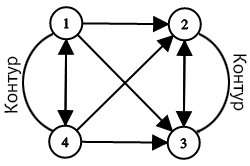
\includegraphics[scale=0.5]{task_1.png}
      \caption*{граф с отмеченными контурами.}
   \end{figure}
   

% %%%%%%%%%%%%%%%%%%%
\section*{Задание 2}
\addcontentsline{toc}{section}{Задание 2}
% %%%%%%%%%%%%%%%%%%%
\begin{figure}[h!]
   \centering
   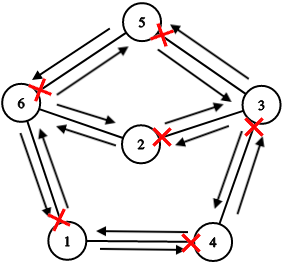
\includegraphics[scale=0.7]{task_2.png}
\end{figure}
$5 \to 6 \to 1 \to 4 \to 3 \to 5 \to 3 \to 2 \to 6 \to 2 \to 3 \to 4 \to 1 \to 6 \to 5$

% %%%%%%%%%%%%%%%%%%%
\section*{Задание 3}
\addcontentsline{toc}{section}{Задание 3}
% %%%%%%%%%%%%%%%%%%%
\begin{minipage}{0.5\textwidth}
$
   \begin{blockarray}{ccccccccc}
      & v_1 & v_2 & v_3 & v_4 & v_5 & v_6 & v_7 \\
      \begin{block}{c(cccccccc)}
      v_1 & 0 & 0 & 0 & 0 & 1 & 1 & 0 \\
      v_2 & 1 & 0 & 1 & 0 & 1 & 1 & 0 \\
      v_3 & 1 & 1 & 0 & 1 & 1 & 0 & 0 \\
      v_4 & 0 & 0 & 1 & 0 & 1 & 1 & 1 \\
      v_5 & 1 & 1 & 0 & 0 & 0 & 1 & 0 \\
      v_6 & 0 & 0 & 1 & 0 & 1 & 0 & 0 \\
      v_7 & 1 & 1 & 0 & 1 & 1 & 0 & 0 \\
      \end{block}
   \end{blockarray}
$
\end{minipage}
\begin{minipage}{0.5\textwidth}
   \begin{tikzpicture}
      \Vertex[x=2, y=3, Math, label=v_1, position=above, fontscale=1.5, size=.2, color=black]{V1};
      \Vertex[x=1, y=2, Math, label=v_5, position=left, fontscale=1.5, size=.2, color=black]{V5};
      \Vertex[x=3, y=2, Math, label=v_6, position=right, fontscale=1.5, size=.2, color=black]{V6};
      \Vertex[x=1, y=1, Math, label=v_2, position=left, fontscale=1.5, size=.2, color=black]{V2};
      \Vertex[x=3, y=1, Math, label=v_3, position=right, fontscale=1.5, size=.2, color=black]{V3};
      \Vertex[x=3, y=0, Math, label=v_4, position=right, fontscale=1.5, size=.2, color=black]{V4};
      \Vertex[x=3, y=-1,Math, label=v_7, position=right, fontscale=1.5, size=.2, color=black]{V7};

      \Text[x=3.5, y=3.2]{$W_0(v_1)$}
      \Text[x=5, y=2]{$W_1(v_1)$}
      \Text[x=5, y=1]{$W_2(v_1)$}
      \Text[x=5, y=0]{$W_3(v_1)$}
      \Text[x=5, y=-1]{$W_4(v_1)$}

      \Edge[Direct](V1)(V5)
      \Edge[Direct](V1)(V6)
      \Edge[Direct](V5)(V2)
      \Edge[Direct](V6)(V3)
      \Edge[Direct](V3)(V4)
      \Edge[Direct](V4)(V7)
   \end{tikzpicture}
\end{minipage}
$v_1 \in W_0$ \\ 
$\Gamma W_1(v_1) = \{ v_5, v_6 \}$ \\
$\Gamma W_2(v_1) = \{ v_2, v_3 \}$ \\
$\Gamma W_3(v_1) = \{ v_4 \}$ \\
$\Gamma W_4(v_1) = \{ v_7 \}$
\begin{enumerate}[leftmargin=*]
   \item $v_7$
   \item $W_3(v_1) \cap \Gamma^{-1}v_7 = \{ v_4 \} \cap \{ v_4 \} = \{ v_4 \}$
   \item $W_2(v_1) \cap \Gamma^{-1}v_4 = \{ v_2, v_3 \} \cap \{ v_7, v_3 \} = \{ v_3 \}$
   \item $W_1(v_1) \cap \Gamma^{-1}v_3 = \{ v_5, v_6 \} \cap \{ v_2, v_4, v_6 \} = \{ v_6 \}$
   \item $W_0(v_1) \cap \Gamma^{-1}v_6 = \{ v_1 \} \cap \{ v_1, v_2, v_4, v_5 \} = \{ v_1 \}$
\end{enumerate}
$v_1 \to v_6 \to v_3 \to v_4 \to v_7$ -- кратчайший путь. Длина кратчайшего пути -- 5.


% %%%%%%%%%%%%%%%%%%%
\section*{Задание 4}
\addcontentsline{toc}{section}{Задание 4}
% %%%%%%%%%%%%%%%%%%%
\begin{center}
   \begin{tabular}{|c|c|c|c|c|c|c|c|c|c|c|c|c|c|c|}
      \hline
      & $v_1$ & $v_2$ & $v_3$ & $v_4$ & $v_5$ & $v_6$ & $v_7$ & $\lambda_i^{(0)}$ & $\lambda_i^{(1)}$ & $\lambda_i^{(2)}$ & $\lambda_i^{(3)}$ & $\lambda_i^{(4)}$ & $\lambda_i^{(5)}$ & $\lambda_i^{(6)}$\\ \hline
      $v_1$ & $\infty$ & 2 & 7 & 8 & $\infty$ & $\infty$ & $\infty$ & \cellcolor{red!35}0\tikzmark{a} & 0 & 0 & 0 & 0 & 0 & 0 \\ \hline 
      $v_2$ & 12 & $\infty$ & 4 & $\infty$ & 6 & $\infty$ & $\infty$ & $\infty$ & \cellcolor{red!35}2\tikzmark{b} & 2 & 2 & 2 & 2 & 2 \\ \hline
      $v_3$ & $\infty$ & 4 & $\infty$ & 1 & 3 & 5 & 7 & $\infty$ & 7 & \cellcolor{red!35}6\tikzmark{c} & 6 & 6 & 6 & 6 \\ \hline
      $v_4$ & $\infty$ & $\infty$ & 1 & $\infty$ & $\infty$ & 3 & $\infty$ & $\infty$ & 8 & 8 & \cellcolor{red!35}7\tikzmark{d} & 7 & 7 & 7 \\ \hline
      $v_5$ & $\infty$ & $\infty$ & 3 & $\infty$ & $\infty$ & $\infty$ & 5 & $\infty$ & $\infty$ & \cellcolor{red!35}8\tikzmark{e} & 8 & 8 & 8 & 8 \\ \hline
      $v_6$ & $\infty$ & $\infty$ & 5 & $\infty$ & $\infty$ & $\infty$ & 2 & $\infty$ & $\infty$ & 11 & 11 & \cellcolor{red!35}10\tikzmark{f} & 10 & 10 \\ \hline
      $v_7$ & 2 & $\infty$ & $\infty$ & 3 & 4 & 6 & 7 & $\infty$ & $\infty$ & 14 & 13 & 13 & \cellcolor{red!35}12\tikzmark{g} & 12 \\ \hline
   \end{tabular}
   \begin{tikzpicture}[overlay, remember picture, yshift=.25\baselineskip]
      \draw[thick,shorten >=10pt, shorten <=1pt] [->] ({pic cs:a}) to ({pic cs:b});
      \draw[thick,shorten >=10pt, shorten <=1pt] [->] ({pic cs:b}) to ({pic cs:c});
      \draw[thick,shorten >=10pt, shorten <=1pt] [->] ({pic cs:c}) to ({pic cs:d});
      \draw[thick,shorten >=13pt, shorten <=1pt] [->] ({pic cs:d}) to ({pic cs:f});
      \draw[thick,shorten >=10pt, shorten <=1pt] [->] ({pic cs:b}) to ({pic cs:e});
      \draw[thick,shorten >=15pt, shorten <=0.1pt] [->] ({pic cs:f}) to ({pic cs:g});
    \end{tikzpicture}
\end{center}
\setlength\parindent{24pt}

\indent Длины минимальных путей из вершины $v_1$ во все остальные вершины определены в последнем столбце таблицы.\\
\indent Найдём вершины, входящие в минимальные пути из $v_1$ во все остальные.\\
1) Минимальный путь из $v_1$ в $v_2$: его длина -- 2\\
$\lambda_1^{(0)} + c_{12} = 0 + 2 = \lambda_2^{(1)}$ \; $v_1 \to v_2$\\[10pt]
2) Минимальный путь из $v_1$ в $v_3$: его длина -- 6\\
$
\begin{rcases*}
\lambda_1^{(0)} + c_{13} = 7 = \lambda_3^{(1)} \; \\
\lambda_2^{(1)} + c_{23} = 2 + 4 = 6 = \lambda_3^{(2)} \;
\end{rcases*} 
$ $min \,\, v_1 \to v_3$ \; $(v_1 \to v_2 \to v_3)$\\[10pt]
3) Минимальный путь из $v_1$ в $v_4$: его длина -- 7\\
$
\begin{rcases*}
   \lambda_3^{(2)} + c_{34} = 6 + 1 = 7 = \lambda_4^{(3)} \; \\
   \lambda_2^{(1)} + c_{23} = 2 + 4 = 6 = \lambda_3^{(2)} \; \\
   \lambda_1^{(0)} + c_{12} = 0 + 2 = 2 = \lambda_2^{(1)} \; \\
\end{rcases*}
$ $min \,\, v_1 \to v_4$ \; $(v_1 \to v_2 \to v_3 \to v_4)$\\[10pt]
4) Минимальный путь из $v_1$ в $v_5$: его длина -- 8\\
$
\begin{rcases*}
   \lambda_2^{(1)} + c_{25} = 2 + 6 = 8 = \lambda_5^{(2)} \; \\
   \lambda_1^{(0)} + c_{12} = 0 + 2 = 2 = \lambda_2^{(1)} \; \\
\end{rcases*}
$ $min \,\, v_1 \to v_5$ \; $(v_1 \to v_2 \to v_5)$\\[10pt]
5) Минимальный путь из $v_1$ в $v_6$: его длина -- 10\\
$
\begin{rcases*}
   \lambda_4^{(3)} + c_{46} = 7 + 3 = 10 = \lambda_6^{(4)} \; \\
   \lambda_3^{(2)} + c_{34} = 6 + 1 = 7 = \lambda_4^{(3)} \; \\
   \lambda_2^{(1)} + c_{23} = 2 + 4 = 6 = \lambda_3^{(2)} \; \\
   \lambda_1^{(0)} + c_{12} = 0 + 2 = 2 = \lambda_2^{(1)} \; \\
\end{rcases*}
$ $min \,\, v_1 \to v_6$ \; $(v_1 \to v_2 \to v_3 \to v_4 \to v_6)$\\[10pt]
6) Минимальный путь из $v_1$ в $v_7$: его длина -- 12\\
$
\begin{rcases*}
   \lambda_6^{(4)} + c_{67} = 10 + 2 = 12 = \lambda_7^{(5)} \; \\
   \lambda_4^{(3)} + c_{46} = 7 + 3 = 10 = \lambda_6^{(4)} \; \\
   \lambda_3^{(2)} + c_{34} = 6 + 1 = 7 = \lambda_4^{(3)} \; \\
   \lambda_2^{(1)} + c_{23} = 2 + 4 = 6 = \lambda_3^{(2)} \; \\
   \lambda_1^{(0)} + c_{12} = 0 + 2 = 2 = \lambda_2^{(1)} \; \\
\end{rcases*}
$
$min \,\, v_1 \to v_7$ \; $(v_1 \to v_2 \to v_3 \to v_4 \to v_6 \to v_7)$\\



% %%%%%%%%%%%%%%%%%%%
\section*{Задание 5}
\addcontentsline{toc}{section}{Задание 5}
% %%%%%%%%%%%%%%%%%%%
\begin{center}
   \begin{minipage}{0.4\textwidth}
      \begin{tikzpicture}[scale=1.5]
         \Vertex[x=0,y=1,fontscale=1.5, size=.2, color=black]{V1};
         \Vertex[x=1,y=1,fontscale=1.5, size=.2, color=black]{V2};
         \Vertex[x=2,y=1,fontscale=1.5, size=.2, color=black]{V3};
         \Vertex[x=3,y=1,fontscale=1.5, size=.2, color=black]{V4};
         \Vertex[x=0,y=0,fontscale=1.5, size=.2, color=black]{V5};
         \Vertex[x=1,y=0,position=right, fontscale=1.5, size=.2, color=black]{V6};
         \Vertex[x=2,y=0,position=right, fontscale=1.5, size=.2, color=black]{V7};
         \Vertex[x=3,y=0,position=right, fontscale=1.5, size=.2, color=black]{V8};
         \Vertex[x=0,y=-1,position=right, fontscale=1.5, size=.2, color=black]{V9};
         \Vertex[x=1,y=-1,position=right, fontscale=1.5, size=.2, color=black]{V10};
         \Vertex[x=2,y=-1,position=right, fontscale=1.5, size=.2, color=black]{V11};
         \Vertex[x=3,y=-1,position=right, fontscale=1.5, size=.2, color=black]{V12};

         \Edge[label=1,fontscale=1.5](V1)(V2)
         \Edge[label=2,fontscale=1.5](V2)(V3)
         \Edge[label=9,fontscale=1.5](V3)(V4)
         \Edge[label=8,fontscale=1.5](V1)(V5)
         \Edge[label=5,fontscale=1.5](V2)(V6)
         \Edge[label=5,fontscale=1.5](V3)(V7)
         \Edge[label=1,fontscale=1.5](V4)(V8)
         \Edge[label=7,fontscale=1.5](V5)(V6)
         \Edge[label=3,fontscale=1.5](V6)(V7)
         \Edge[label=8,fontscale=1.5](V7)(V8)
         \Edge[label=2,fontscale=1.5](V5)(V9)
         \Edge[label=5,fontscale=1.5](V6)(V10)
         \Edge[label=5,fontscale=1.5](V7)(V11)
         \Edge[label=5,fontscale=1.5](V8)(V12)
         \Edge[label=6,fontscale=1.5](V9)(V10)
         \Edge[label=4,fontscale=1.5](V10)(V11)
         \Edge[label=4,fontscale=1.5](V11)(V12)
      \end{tikzpicture}
   \end{minipage}
   \begin{minipage}{0.4\textwidth}
      \begin{tikzpicture}[scale=1.5]
         \Vertex[x=0,y=1,fontscale=1.5, size=.2, color=black]{V1};
         \Vertex[x=1,y=1,fontscale=1.5, size=.2, color=black]{V2};
         \Vertex[x=2,y=1,fontscale=1.5, size=.2, color=black]{V3};
         \Vertex[x=3,y=1,fontscale=1.5, size=.2, color=black]{V4};
         \Vertex[x=0,y=0,fontscale=1.5, size=.2, color=black]{V5};
         \Vertex[x=1,y=0,position=right, fontscale=1.5, size=.2, color=black]{V6};
         \Vertex[x=2,y=0,position=right, fontscale=1.5, size=.2, color=black]{V7};
         \Vertex[x=3,y=0,position=right, fontscale=1.5, size=.2, color=black]{V8};
         \Vertex[x=0,y=-1,position=right, fontscale=1.5, size=.2, color=black]{V9};
         \Vertex[x=1,y=-1,position=right, fontscale=1.5, size=.2, color=black]{V10};
         \Vertex[x=2,y=-1,position=right, fontscale=1.5, size=.2, color=black]{V11};
         \Vertex[x=3,y=-1,position=right, fontscale=1.5, size=.2, color=black]{V12};

         \Edge[Math,label=x_3,position=above,fontscale=1.5](V1)(V2)
         \Edge[Math,label=x_8,position=above,fontscale=1.5](V2)(V3)
         \Edge[Math,label=x_{16},position=right,fontscale=1.5](V3)(V7)
         \Edge[Math,label=x_{13},position=right,fontscale=1.5](V4)(V8)
         \Edge[Math,label=x_7,position=above,fontscale=1.5](V6)(V7)
         \Edge[Math,label=x_1,position=left,fontscale=1.5](V5)(V9)
         \Edge[Math,label=x_{15},position=right,fontscale=1.5](V6)(V10)
         \Edge[Math,label=x_{12},position=right,fontscale=1.5](V8)(V12)
         \Edge[Math,label=x_5,position=below,fontscale=1.5](V9)(V10)
         \Edge[Math,label=x_6,position=below,fontscale=1.5](V10)(V11)
         \Edge[Math,label=x_{11},position=below,fontscale=1.5](V11)(V12)
      \end{tikzpicture}
   \end{minipage}
\end{center}
\begin{enumerate}[leftmargin=*,itemsep=0.1ex]
   \item $x_3, x_{13}$ -- 1 (нет циклов)
   \item $x_1, x_8$ -- 2 (нет циклов)
   \item $x_7$ -- 3 (нет циклов)
   \item $x_6, x_{11}$ -- 4 (нет циклов)
   \item $x_{16}, x_{15}, x_{12}$ -- 5 (т.к. если добавить все «5» будет цикл)
   \item $x_5$ -- 6
\end{enumerate}
$L(D) = 1\cdot2 + 2\cdot2 + 3\cdot1 + 4\cdot2 + 5\cdot3 + 6 = 38$ -- минимальный вес остовного дерева.


% %%%%%%%%%%%%%%%%%%%
\section*{Задание 6}
\addcontentsline{toc}{section}{Задание 6}
% %%%%%%%%%%%%%%%%%%%
   \begin{minipage}{0.4\textwidth}
      \begin{tikzpicture}[scale=2]
         \Vertex[Math,label=v_1,position=above,x=0,y=0,opacity=0,color=black,size=.5,fontscale=1.5]{v1}
         \Vertex[Math,label=v_2,position=above,x=2,y=0,opacity=0,color=black,size=.5,fontscale=1.5]{v2}
         \Vertex[Math,label=v_3,position=left,x=0,y=-1,opacity=0,color=black,size=.5,fontscale=1.5]{v3}
         \Vertex[Math,label=v_4,position=below,x=1,y=-1,opacity=0,color=black,size=.5,fontscale=1.5]{v4}
         \Vertex[Math,label=v_5,position=right,x=2,y=-1,opacity=0,color=black,size=.5,fontscale=1.5]{v5}
         \Vertex[Math,label=v_6,position=below,x=0,y=-2,opacity=0,color=black,size=.5,fontscale=1.5]{v6}
         \Vertex[Math,label=v_7,position=below,x=2,y=-2,opacity=0,color=black,size=.5,fontscale=1.5]{v7}

         \Edge[Direct,label=2,fontscale=1.3,color=black](v1)(v2)
         \Edge[Direct,label=1,fontscale=1.3,color=black](v1)(v3)
         \Edge[Direct,label=8,fontscale=1.3,color=black](v1)(v4)
         \Edge[Direct,label=7,fontscale=1.3,color=black](v2)(v3)
         \Edge[Direct,label=12,fontscale=1.3,color=black](v3)(v4)
         \Edge[Direct,label=6,fontscale=1.3,color=black](v3)(v6)
         \Edge[Direct,label=11,fontscale=1.3,color=black](v4)(v5)
         \Edge[Direct,label=13,fontscale=1.3,color=black](v4)(v2)
         \Edge[Direct,label=9,fontscale=1.3,color=black](v4)(v6)
         \Edge[Direct,label=3,fontscale=1.3,color=black](v5)(v2)
         \Edge[Direct,label=4,fontscale=1.3,color=black](v5)(v7)
         \Edge[Direct,label=5,fontscale=1.3,color=black](v6)(v7)
         \Edge[Direct,label=10,fontscale=1.3,color=black](v7)(v4)
      \end{tikzpicture}
   \end{minipage}
   \begin{minipage}{0.6\textwidth}
   \begin{enumerate}[leftmargin=*]
      \item $D_1 = (v_{i1}, \varnothing)$
      \item $D_2 = (\{v_{i1},v_{i2}\},\{v_{i1},v_{i2}\})$
      \item $D_3 = (\{v_{i1},v_{i2},v_{i3}\},\{v_{i1},v_{i2}\},\{v_{i2},v_{i3}\})$
      \item $D_4 = D_3 + \{v_{i4}\} + \{v_{i3},v_{i4}\}$
      \item $D_5 = D_4 + \{v_{i5}\} + \{v_{i4},v_{i5}\}$
      \item $D_6 = D_5 + \{v_{i7}\} + \{v_{i5},v_{i7}\}$
      \item $D_7 = D_6 + \{v_{i6}\} + \{v_{i4},v_{i6}\}$
   \end{enumerate}
   \end{minipage}\\[40pt]
   \begin{minipage}{0.6\textwidth}
      \begin{enumerate}[leftmargin=*]
         \item $(D + q_1):\mu_1:v_1 - v_2 - v_3 - v_1 \implies c(\mu_1) = (\begin{array}{*{13}c}-1 & 1 & 0 & 0 & 0 & 0 & 1 & 0 & 0 & 0 & 0 & 0 & 0\end{array})$
         \item $(D + q_3):\mu_2:v_2 - v_3 - v_4 - v_5 - v_2 \implies c(\mu_2) = (\begin{array}{*{13}c}0 & 0 & 1 & 0 & 0 & 0 & 1 & 0 & 0 & 0 & 1 & 1 & 0\end{array})$
         \item $(D + q_5):\mu_3:v_4 - v_5 - v_7 - v_6 - v_4 \implies c(\mu_3) = (\begin{array}{*{13}c}0 & 0 & 0 & 1 & -1 & 0 & 0 & 0 & -1 & 0 & 1 & 0 & 0\end{array})$
         \item $(D + q_6):\mu_4:v_3 - v_4 - v_6 - v_3 \implies c(\mu_4) = (\begin{array}{*{13}c}0 & 0 & 0 & 0 & 0 & -1 & 0 & 0 & 1 & 0 & 0 & 1 & 0\end{array})$ 
         \item $(D + q_8):\mu_5:v_1 - v_2 - v_3 - v_4 - v_1 \implies c(\mu_5) = (\begin{array}{*{13}c}0 & 1 & 0 & 0 & 0 & 0 & 1 & -1 & 0 & 0 & 0 & 1 & 0\end{array})$ 
         \item $(D + q_{10}):\mu_6:v_4 - v_5 - v_7 - v_4 \implies c(\mu_6) = (\begin{array}{*{13}c}0 & 0 & 0 & 1 & 0 & 0 & 0 & 0 & 0 & 1 & 1 & 0 & 0\end{array})$ 
         \item $(D + q_{13}):\mu_7:v_2 - v_3 - v_4 - v_2 \implies c(\mu_7) = (\begin{array}{*{13}c}0 & 0 & 0 & 0 & 0 & 0 & 1 & 0 & 0 & 0 & 0 & 1 & 1\end{array})$ 
      \end{enumerate}
   \end{minipage}
   \hspace{20pt}
   \begin{minipage}{0.4\textwidth}
      \begin{tikzpicture}[scale=2]
         \Vertex[Math,label=v_1,position=above,x=0,y=0,opacity=0,color=black,size=.5,fontscale=1.5]{v1}
         \Vertex[Math,label=v_2,position=above,x=2,y=0,opacity=0,color=black,size=.5,fontscale=1.5]{v2}
         \Vertex[Math,label=v_3,position=left,x=0,y=-1,opacity=0,color=black,size=.5,fontscale=1.5]{v3}
         \Vertex[Math,label=v_4,position=below,x=1,y=-1,opacity=0,color=black,size=.5,fontscale=1.5]{v4}
         \Vertex[Math,label=v_5,position=right,x=2,y=-1,opacity=0,color=black,size=.5,fontscale=1.5]{v5}
         \Vertex[Math,label=v_6,position=below,x=0,y=-2,opacity=0,color=black,size=.5,fontscale=1.5]{v6}
         \Vertex[Math,label=v_7,position=below,x=2,y=-2,opacity=0,color=black,size=.5,fontscale=1.5]{v7}

         \Edge[Direct,Math,label=q_2,fontscale=1.3,color=black](v1)(v2)
         \Edge[Direct,Math,label=q_7,fontscale=1.3,color=black](v2)(v3)
         \Edge[Direct,Math,label=q_{12},fontscale=1.3,color=black](v3)(v4)
         \Edge[Direct,Math,label=q_{11},fontscale=1.3,color=black](v4)(v5)
         \Edge[Direct,Math,label=q_9,fontscale=1.3,color=black](v4)(v6)
         \Edge[Direct,Math,label=q_4,fontscale=1.3,color=black](v5)(v7)
      \end{tikzpicture}
   \end{minipage} \\[20pt]
Цикломатическая матрица C: \\
$$
\begin{pmatrix}
   -1 & 1 & 0 & 0 & 0 & 0 & 1 & 0 & 0 & 0 & 0 & 0 & 0 \\
   0 & 0 & 1 & 0 & 0 & 0 & 1 & 0 & 0 & 0 & 1 & 1 & 0 \\
   0 & 0 & 0 & 1 & -1 & 0 & 0 & 0 & -1 & 0 & 1 & 0 & 0 \\
   0 & 0 & 0 & 0 & 0 & -1 & 0 & 0 & 1 & 0 & 0 & 1 & 0 \\
   0 & 1 & 0 & 0 & 0 & 0 & 1 & -1 & 0 & 0 & 0 & 1 & 0 \\
   0 & 0 & 0 & 1 & 0 & 0 & 0 & 0 & 0 & 1 & 1 & 0 & 0 \\
   0 & 0 & 0 & 0 & 0 & 0 & 1 & 0 & 0 & 0 & 0 & 1 & 1
\end{pmatrix}
$$ \\[10pt]
Закон Кирхгофа для напряжений: \\
$$
   C \cdot \begin{pmatrix}
      u_1 \\
      \vdots \\
      u_{13}
   \end{pmatrix} = 0 \implies \begin{cases}
      -u_1 + u_2 + u_7 = 0 \\
      u_3 + u_7 + u_{11} + u_{12} = 0 \\
      u_4 - u_5 - u_9 + u_{11} = 0 \\
      -u_6 + u_9 + u_{12} = 0 \\
      u_7 - u_8 + u_{12} = 0 \\
      u_4 + u_{10} + u_{11} = 0 \\
      u_7 + u_{12} + u_{13}= 0
   \end{cases} \implies \begin{cases}
      u_1 = u_2 + u_7 \\
      u_3 = -u_7 - u_{11} - u_{12} \\
      u_5 = u_4 - u_9 + u_{11} \\
      u_6 = u_9 + u_{12} \\
      u_8 = u_7 + u_{12} \\
      u_{10} = -u_4 - u_{11} \\
      u_{13} = -u_7 - u_{12}
   \end{cases}
$$
Выпишем уравнения Кирхгофа для токов. Найдём матрицу инцидентности B орграфа: \\
\begin{center}
\begin{blockarray}{|c|c|c|c|c|c|c|c|c|c|c|c|c|c|}
   \hline
   & $q_1$ & $q_2$ & $q_3$ & $q_4$ & $q_5$ & $q_6$ & $q_7$ & $q_8$ & $q_9$ & $q_{10}$ & $q_{11}$ & $q_{12}$ & $q_{13}$ \\ \hline
   $v_1$ & -1 & -1 & 0 & 0 & 0 & 0 & 0 & -1 & 0 & 0 & 0 & 0 & 0 \\ \hline
   $v_2$ & 0 & 1 & 1 & 0 & 0 & 0 & -1 & 0 & 0 & 0 & 0 & 0 & 1 \\ \hline
   $v_3$ & 1 & 0 & 0 & 0 & 0 & -1 & 1 & 0 & 0 & 0 & 0 & -1 & 0 \\ \hline
   $v_4$ & 0 & 0 & 0 & 0 & 0 & 0 & 0 & 1 & -1 & 1 & -1 & 1 & -1 \\ \hline
   $v_5$ & 0 & 0 & -1 & -1 & 0 & 0 & 0 & 0 & 0 & 0 & 1 & 0 & 0 \\ \hline
   $v_6$ & 0 & 0 & 0 & 0 & -1 & 1 & 0 & 0 & 1 & 0 & 0 & 0 & 0 \\ \hline
   $v_7$ & 0 & 0 & 0 & 1 & 1 & 0 & 0 & 0 & 0 & -1 & 0 & 0 & 0 \\ \hline
\end{blockarray}
\end{center}
\begin{equation}
   B \cdot \begin{pmatrix}
      I_1 \\
      \vdots \\
      I_{13}
   \end{pmatrix} = 0 \implies \begin{cases}
      I_1 + I_2 + I_8 = 0 \\
      I_2 + I_3 - I_7 + I_{13} = 0 \\
      I_1 - I_6 + I_7 - I_{12} = 0 \\
      \hbox{\sout{$I_8 - I_9 + I_{10} - I_{11} + I_{12} - I_{13} = 0$}} \\
      I_{11} - I_3 - I_4 = 0 \\
      I_7 - I_6 + I_9 = 0 \\
      I_5 + I_6 - I_{10}
   \end{cases}
\end{equation} \\
\begin{equation}
   \begin{cases}
      E_1 = I_2R_2 + I_7R_7 \\
      E_2 = I_4R_4 - I_9R_9 + I_{11}R_{11} \\
      I_3R_3 + I_7R_7 + I_{11}R_{11} + I_{12}R_{12} = 0 \\
      I_6R_6 - I_9R_9 - I_{12}R_{12} = 0 \\
      I_8R_8 - I_7R_7 - I_{12}R_{12} = 0 \\
      I_{10}R_{10} + I_4R_4 + I_{11}R_{11} = 0 \\
      I_{13}R_{13} + I_7R_7 + I_{12}R_{12} = 0
   \end{cases}
\end{equation}
Совместная система состоит из систем (1) и (2). 13 уравнений из 13 неизвестных -- токи $I_1 \dots I_{13}; \, E_1, E_2, R_2, R_3, R_4, R_6, R_7, R_8, R_9, R_{10}, R_{11}, R_{12}, R_{13}$ -- известны.


% %%%%%%%%%%%%%%%%%%
\section*{Задание 7}
\addcontentsline{toc}{section}{Задание 7}
% %%%%%%%%%%%%%%%%%%%
\begin{minipage}[h!]{0.6\textwidth}
   \begin{tikzpicture}
      % \SetVertexStyle[TextFont=1.5]
      \Vertex[x=0,y=0,size=.2,color=black,Math,label=v_1,position=above,fontscale=1.5]{v1}
      \Vertex[x=2,y=1,size=.2,color=black,Math,label=v_2,position=above,fontscale=1.5]{v2}
      \Vertex[x=4,y=2,size=.2,color=black,Math,label=v_3,position=above,fontscale=1.5]{v3}
      \Vertex[x=6,y=1,size=.2,color=black,Math,label=v_4,position=above,fontscale=1.5]{v4}
      \Vertex[x=8,y=0,size=.2,color=black,Math,label=v_5,position=above,fontscale=1.5]{v5}
      \Vertex[x=2,y=-1,size=.2,color=black,Math,label=v_8,position=below,fontscale=1.5]{v8}
      \Vertex[x=4,y=-2,size=.2,color=black,Math,label=v_7,position=below,fontscale=1.5]{v7}
      \Vertex[x=6,y=-1,size=.2,color=black,Math,label=v_6,position=below,fontscale=1.5]{v6}
      \Vertex[x=4,y=0,size=.2,color=black,Math,label=v_9,position=above,fontscale=1.5]{v9}

      \SetEdgeStyle[Color=black]
      \Edge[Direct,label=6,fontscale=1.2](v1)(v2)
      \Edge[Direct,label=6,fontscale=1.2](v2)(v3)
      \Edge[Direct,label=7,fontscale=1.2](v3)(v4)
      \Edge[Direct,label=9,fontscale=1.2](v4)(v5)
      \Edge[Direct,label=6,fontscale=1.2](v1)(v9)
      \Edge[Direct,label=5,fontscale=1.2](v9)(v5)
      \Edge[Direct,label=3,fontscale=1.2](v1)(v8)
      \Edge[Direct,label=3,fontscale=1.2](v8)(v7)
      \Edge[Direct,label=9,fontscale=1.2](v7)(v6)
      \Edge[Direct,label=16,fontscale=1.2](v6)(v5)
      \Edge[Direct,label=2,fontscale=1.2](v2)(v9)
      \Edge[Direct,label=3,fontscale=1.2](v9)(v4)
      \Edge[Direct,label=7,fontscale=1.2](v8)(v9)
      \Edge[Direct,label=6,fontscale=1.2](v9)(v6)
      \Edge[Direct,label=8,bend=-25,fontscale=1.2,distance=.8](v1)(v3)
      \Edge[Direct,label=9,bend=25,fontscale=1.2,distance=.8](v1)(v7)
   \end{tikzpicture}
\end{minipage}
\begin{minipage}[r]{0.4\textwidth}
   Поиск полного потока:\\
   $v_1 \to v_2 \to v_3 \to v_4 \to v_5: \, min = 6$ \\
   $v_1 \to v_8 \to v_7 \to v_6 \to v_5: \, min = 3$ \\
   $v_1 \to v_9 \to v_5: \, min = 5$ \\
   насытили $<v_1,v_2>, <v_2,v_3>, \\ <v_9,v_5>, <v_1,v_8>, <v_8,v_7>$ \\
   $v_1 \to v_3 \to v_4 \to v_5 \implies$ \\
   \small{$\{8;7-6;9-6\} \implies min = 1$} \\
   насытили $<v_3,v_4>$ \\
   $v_1 \to v_7 \to v_6 \to v_5$ \\
   \small{$\{9;9-3;16-3\} \implies min = 6$} \\
   насытили $<v_7,v_6>$ \\
   $v_1 \to v_9 \to v_4 \to v_5$ \\
   \small{$\{6-5;3;9-7\} \implies min = 1$} \\
   насытили $<v_1,v_9>$
\end{minipage} \\[10pt]
\begin{minipage}{0.5\textwidth}
   Проверим, что $\sum{c_f(s,u)} = \sum{c_f(u,t)} : \\ v_1 - s, v_5 - t$. \\
   $6 + 1 + 6 + 6 + 3 = 8 + 5 + 9 \implies 22 = 22 \implies$ всё сходится. \\
   $\Phi_\textup{полн.} = 22 = 8 + 5 + 9$
\end{minipage}
\begin{center}
   \begin{tikzpicture}
      \Vertex[x=0,y=0,size=.2,color=black,Math,label=v_1,position=above,fontscale=1.5]{v1}
      \Vertex[x=2,y=1,size=.2,color=black,Math,label=v_2,position=above,fontscale=1.5]{v2}
      \Vertex[x=4,y=2,size=.2,color=black,Math,label=v_3,position=above,fontscale=1.5]{v3}
      \Vertex[x=6,y=1,size=.2,color=black,Math,label=v_4,position=above,fontscale=1.5]{v4}
      \Vertex[x=8,y=0,size=.2,color=black,Math,label=v_5,position=above,fontscale=1.5]{v5}
      \Vertex[x=2,y=-1,size=.2,color=black,Math,label=v_8,position=below,fontscale=1.5]{v8}
      \Vertex[x=4,y=-2,size=.2,color=black,Math,label=v_7,position=below,fontscale=1.5]{v7}
      \Vertex[x=6,y=-1,size=.2,color=black,Math,label=v_6,position=below,fontscale=1.5]{v6}
      \Vertex[x=4,y=0,size=.2,color=black,Math,label=v_9,position=above,fontscale=1.5]{v9}

      \SetEdgeStyle[Color=black]
      \Edge[Direct,Math,label=0+6,fontscale=0.8,color=red](v1)(v2)
      \Edge[Direct,Math,label=0+6,fontscale=0.8,color=red](v2)(v3)
      \Edge[Direct,Math,label=0+6+1,fontscale=0.8,color=red](v3)(v4)
      \Edge[Direct,Math,label=0+6+1+1,fontscale=0.8](v4)(v5)
      \Edge[Direct,Math,label=0+6,fontscale=0.8,color=red](v1)(v9)
      \Edge[Direct,Math,label=0+5,fontscale=0.8,color=red](v9)(v5)
      \Edge[Direct,Math,label=0+3,fontscale=0.8,color=red](v1)(v8)
      \Edge[Direct,Math,label=0+3,fontscale=0.8,color=red](v8)(v7)
      \Edge[Direct,Math,label=0+6+3,fontscale=0.8,color=red](v7)(v6)
      \Edge[Direct,Math,label=0+6+3,fontscale=0.8](v6)(v5)
      \Edge[Direct,Math,fontscale=0.8](v2)(v9)
      \Edge[Direct,Math,label=0+1,fontscale=0.8](v9)(v4)
      \Edge[Direct,Math,fontscale=0.8](v8)(v9)
      \Edge[Direct,Math,fontscale=0.8](v9)(v6)
      \Edge[Direct,Math,label=0+1,bend=-25,fontscale=0.8,distance=.9,position=below](v1)(v3)
      \Edge[Direct,Math,label=0+6,bend=25,fontscale=0.8,distance=.9,position=above](v1)(v7)

      % \Text[x=1.5,y=0.8,RGB,color={255,0,0}]{\textbf{X}}
      % \Text[x=1.5,y=0.8,RGB,color={255,0,0}]{\textbf{X}}
      % \Text[x=1.5,y=0.8,RGB,color={255,0,0}]{\textbf{X}}
      % \Text[x=1.5,y=0.8,RGB,color={255,0,0}]{\textbf{X}}
   \end{tikzpicture}
\end{center}
Теперь будем строить максимальный поток \\
1. 
\small{$v_1 \to v_3 \to v_2 \to v_9 \to v_4 \to v_5; \, min = 1 \, (<v_4,v_5>) \implies \\
   % <v_4,v_5>: + 1 \implies 9/9 \\
   % <v_9,v_4>: + 1 \implies 3/2 \\
   % <v_1,v_3>: + 1 \implies 8/2 \\
   % <v_2,v_3>: - 1 \implies 6/5 \\
   % <v_2,v_9>: + 1 \implies 2/1 \\[10pt]
$} $\triangle_1 = min\{8-1,\, \underline{6},\, 2,\, 2-1,\, 9-8\} = 1$ \\[10pt]
2. Далее
\small{$
   v_1 \to v_3 \to v_2 \to v_9 \to v_6 \to v_5; \, min = 1 \, (<v_2,v_9>) \implies \\
   % <v_1,v_3>: + 1 \implies 8/3 \\
   % <v_2,v_3>: - 1 \implies 6/4 \\
   % <v_2,v_9>: + 1 \implies 2/2 \\
   % <v_9,v_6>: + 1 \implies 6/1 \\
   % <v_6,v_5>: + 1 \implies 16/10 \\[10pt]
$} $\triangle_2 = min\{8-2,\, \underline{5},\, 2-1,\, 4,\, 16-9\} = 1$ \\[10pt]
3.
\small{$
   v_1 \to v_7 \to v_8 \to v_9 \to v_6 \to v_5; \, min = 3 \, (<v_1,v_7>) \implies \\
   % <v_1,v_7>: + 3 \implies 9/9 \\
   % <v_8,v_7>: - 3 \implies 3 \\
   % <v_8,v_9>: + 3 \implies 7/3 \\
   % <v_9,v_6>: + 3 \implies 6/4 \\
   % <v_6,v_5>: + 3 \implies 16/13 \\[10pt]
$} $\triangle_3 = min\{9-6,\, \underline{3},\, \underline{7},\, 6-1,\, 16-9\} = 3$ \\[10pt]
\normalsize{
% 4. Ненасыщенных дуг больше не осталось, которые образовывали бы путь из $s$ в $t$. \\[10pt]
\begin{center}
   \begin{tikzpicture}
      \Vertex[x=0,y=0,size=.2,color=black,Math,label=v_1,position=above,fontscale=1.5]{v1}
      \Vertex[x=2,y=1,size=.2,color=black,Math,label=v_2,position=above,fontscale=1.5]{v2}
      \Vertex[x=4,y=2,size=.2,color=black,Math,label=v_3,position=above,fontscale=1.5]{v3}
      \Vertex[x=6,y=1,size=.2,color=black,Math,label=v_4,position=above,fontscale=1.5]{v4}
      \Vertex[x=8,y=0,size=.2,color=black,Math,label=v_5,position=above,fontscale=1.5]{v5}
      \Vertex[x=2,y=-1,size=.2,color=black,Math,label=v_8,position=below,fontscale=1.5]{v8}
      \Vertex[x=4,y=-2,size=.2,color=black,Math,label=v_7,position=below,fontscale=1.5]{v7}
      \Vertex[x=6,y=-1,size=.2,color=black,Math,label=v_6,position=below,fontscale=1.5]{v6}
      \Vertex[x=4,y=0,size=.2,color=black,Math,label=v_9,position=above,fontscale=1.5]{v9}

      \SetEdgeStyle[Color=black]
      \Edge[Direct,label=6,fontscale=0.9,color=red](v1)(v2)
      \Edge[Direct,label=6-1-1,fontscale=0.9,color=red](v2)(v3)
      \Edge[Direct,label=7,fontscale=0.9,color=red](v3)(v4)
      \Edge[Direct,label=8+1,fontscale=0.9,color=red](v4)(v5)
      \Edge[Direct,label=6,fontscale=0.9,color=red](v1)(v9)
      \Edge[Direct,label=5,fontscale=0.9,color=red](v9)(v5)
      \Edge[Direct,label=3,fontscale=0.9,color=red](v1)(v8)
      \Edge[Direct,label=3-3,fontscale=0.9,color=red](v8)(v7)
      \Edge[Direct,label=9,fontscale=0.9,color=red](v7)(v6)
      \Edge[Direct,label=9+1+3,fontscale=0.9](v6)(v5)
      \Edge[Direct,label=0+1+1,fontscale=0.9,color=red](v2)(v9)
      \Edge[Direct,label=1+1,fontscale=0.9](v9)(v4)
      \Edge[Direct,label=0+3,fontscale=0.9](v8)(v9)
      \Edge[Direct,label=1+3,fontscale=0.9](v9)(v6)
      \Edge[Direct,label=1+1+1,bend=-25,fontscale=0.9,distance=.75,position=right](v1)(v3)
      \Edge[Direct,label=6+3,bend=25,fontscale=0.9,distance=.75,position=right,color=red](v1)(v7)

   \end{tikzpicture}
\end{center}
Проверим, что $\sum{c_f(s,u)} = \sum{c_f(u,t)} :$ \\
$6 + 3 + 6 + 9 + 3 = 9 + 5 + 13 \implies 27= 27 \implies$ всё сходится. \\
$\Phi_\textup{макс.} = 27 = 9 + 5 + 13$ \\
Следовательно величина $|f|$ максимального потока равна 27.
}

\pagebreak

% %%%%%%%%%%%%%%%%%%%
\section*{Задание 8}
\addcontentsline{toc}{section}{Задание 8}
% %%%%%%%%%%%%%%%%%%%
\begin{center}
   \textbf{Теоретические сведения.}
\end{center}
\setlength\parindent{24pt}

\indent Гиперграф $(H)$ -- обобщение простого графа, когда рёбрами могут быть не только двухэлементные, но и любые подмножества вершин. \\
Пусть $V$ -- конечное непустое множество, $E$ -- некоторое семейство непустых различных подмножеств множества $V$. Пара $(V,E)$ называется гиперграфом с множеством \textit{вершин} $V$ и множеством \textit{рёбер} $E$.\\
\indent Если вершина $v \in V$ принадлежит ребру $e \in E$, то будем говорить, что они \textit{инцидентны}. Число $|E(v)|$ называется степенью вершины $v$, а $|e|$ -- степенью ребра $e$. Вершина гиперграфа, не инцидентная никакому ребру, называется \textit{изолированной}.\\
\indent Для любого гиперграфа можно определить граф инциденций -- \textit{двудольный} граф с множеством вершин $V \cup E$ и множеством рёбер $\{(v,e):(v,e) \in V \times E, v \in e \}$.\\
\indent Для гиперграфов также существует понятие вершинной раскраски. Раскраску вершин гиперграфа будем называть \textit{правильной}, если любые две вершины $v_i,v_j$, принадлежащие одному ребру $e_t$ $v_i, v_j \in e_t, i \ne j$ имеют разные цвета.\\
\indent \textit{Хроматическое число} $\chi(H)$ -- наименьшее число цветов, достаточное для правильной раскраски гиперграфа H.\\
\indent \textit{Двудольный граф} -- граф, множество вершин которого можно разбить на две части таким образом, что каждое ребро графа соединяет какую-то вершину из одной части с какой-то вершиной другой части, то есть не существует ребра, соединяющего две вершины из одной и той же части. \\[10pt]

\begin{center}
   \textbf{Описание алгоритма.}
\end{center}
\setlength\parindent{24pt}

\indent Гиперграф задаётся с помощью матрицы инцидентности, где 1 -- означает принадлежность к ребру, а 0 -- отсутствие принадлежности. \\
\indent Сперва следует преобразовать матрицу инцидентности в список смежности вершин и упорядочить его.
\begin{enumerate}[leftmargin=*]
   \item Построить список смежности вершин.
   \item Упорядочить по убыванию степеней (количество рёбер, содержащих данную вершину).
\end{enumerate}
Затем следует непосредственно раскраска:
\begin{enumerate}[leftmargin=*,label*=\arabic*.]
   \item Окрасить первую вершину в цвет 1.
   \item Выбрать цвет окраски 1.
   \item Пока не окрашены все вершины, повторять п. 3.1 -- 3.2:
   \begin{enumerate}[label*=\arabic*.]
      \item Окрасить в выбранный цвет всякую вершину, которая не смежна с другой, уже окрашенной в этот цвет.
      \item Выбрать следующий цвет.
   \end{enumerate}
\end{enumerate}

\begin{center}
   \textbf{Логическая блок-схема алгоритма.}
\end{center}
\begin{center}
   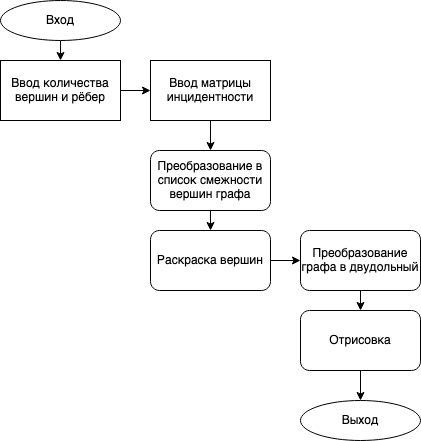
\includegraphics[scale=0.8]{block-scheme.png}
\end{center}
\setlength\parindent{24pt}

\indent Программа написана на языке Python с помощью библиотеки Qt (PyQt), а также Networkx, для создания интерфейса и отрисовки графа соответственно.

\begin{center}
   \textbf{Оценка сложности алгоритма.}
\end{center}
\setlength\parindent{24pt}

\indent Не учитывая время, затраченное на сортировку вершин в порядке невозрастания степеней, необходимо сделать цикл по всем вершинам гиперграфа. Для каждой необходимо найти минимальный цвет, что в худшем случае может занять $O(V^2)$. Значит, общее время составит $O(V^3)$ в худшем случае.

\begin{center}
   \textbf{Тестовые примеры. Скриншоты программ.}
\end{center}
\textbf{Пример 1.} Вводится частный случай гиперграфа с 7 вершинами и 11 рёбрами. Граф представлен на рис. 1.
\begin{center}
   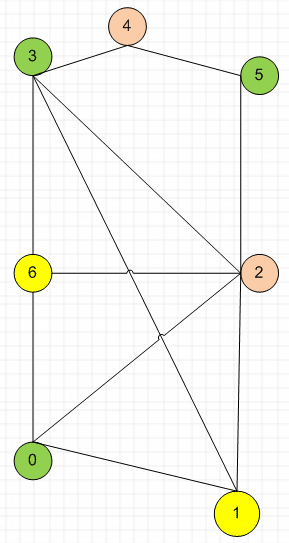
\includegraphics[scale=0.8]{sample-1_1.png} \\
   \captionof{figure}{Частный случай гиперграфа}
   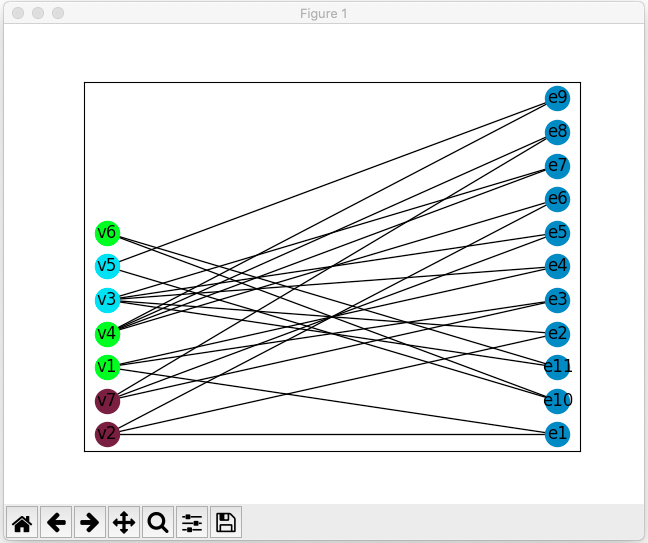
\includegraphics[scale=0.6]{sample-1_2.png}
   \captionof{figure}{Представление графа в виде двудольного\\[10pt]}
   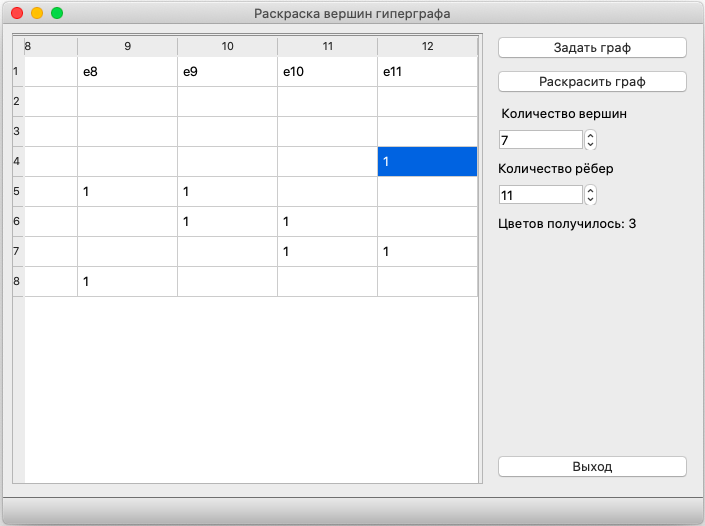
\includegraphics[scale=0.6]{sample-1_3.png}
   \captionof{figure}{Вид программы и матрица инцидентности\\[20pt]}
\end{center}

\textbf{Пример 2.} Дан гипеграф с 6 вершинами и 3 рёбрами.
\begin{center}
   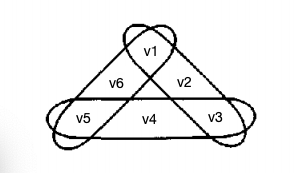
\includegraphics[scale=0.8]{sample-2_1.png} \\
   \captionof{figure}{Гиперграф\\[10pt]}
   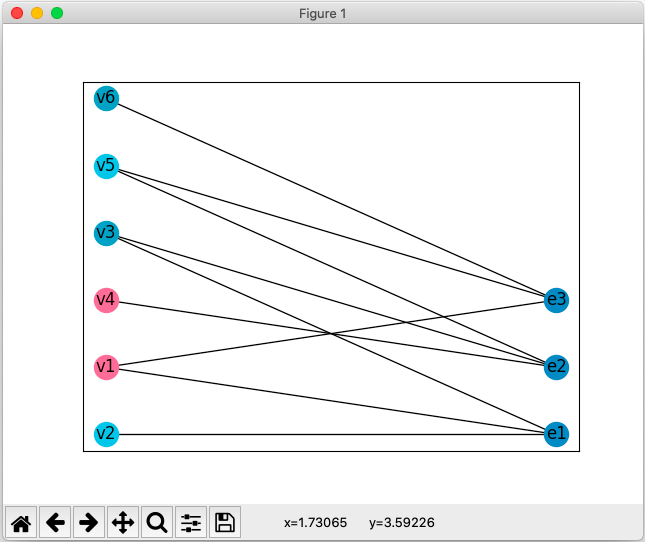
\includegraphics[scale=0.6]{sample-2_2.png}
   \captionof{figure}{Представление графа в виде двудольного\\[10pt]}
   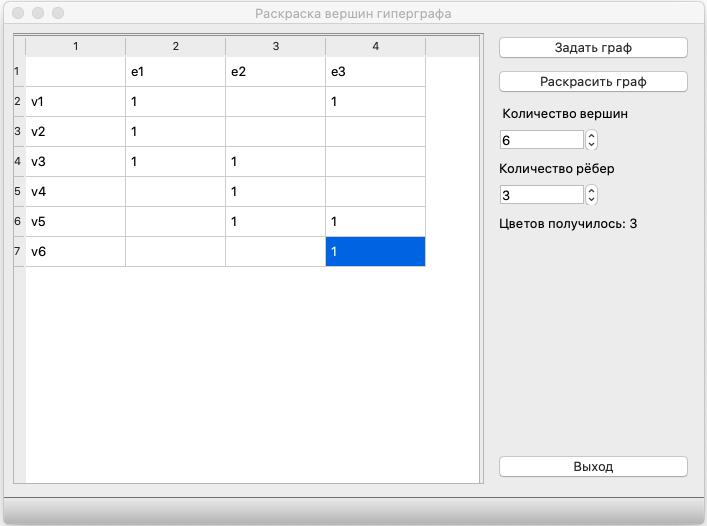
\includegraphics[scale=0.6]{sample-2_3.png}
   \captionof{figure}{Вид программы и матрица инцидентности}
\end{center}

\begin{center}
   \textbf{Примеры прикладных задач.}
\end{center}
\setlength\parindent{24pt}

\indent Для частного случая гиперграфа, например: в задачах календарного планирования осмотры представляются в виде временных интервалов.
Каждому осмотру можно сопоставить вершину графа, причём две любые вершины будут соединены ребром только тогда, когда соответствующие им осмотры нелья осуществлять одновременно.
Требуется составить такой график осмотра, который связан с наименьшыми временными затратами. Задача эквивалентна задаче о раскраске вершин графа с использованием наименьшего числа цветов.\\
\indent Для гиперграфа можно положить следующую общую задачу: имеется $N$ человек с разными навыками. Есть также $K$ умений, которыми они владеют и всех людей надо разбить на $K$ групп по $L$ человек лучших в этом деле. Например, распределить сбалансированные группы для работы над разными проектами.
Пусть каждому элементу из $N$ соответствует какой-то цвет. Тогда вопрос можно сформулировать так: всегда ли существует раскраска в $t$ цветов, при которой группы по $L$ человек будут "неодноцветны"?
Такая задача является более общей задачей, однако мы можем находить минмальное возможное количество цветов, при которых эти условия выполнены.

\pagebreak

\addcontentsline{toc}{section}{Литература}
\begin{thebibliography}{9}
   \bibitem{christofides}
   Никос Кристофидес. Теория графов: алгоритмический подход. М.: Мир, 1978. - 423 стр.

   \bibitem{emelichev}
   Емеличев В.А., Мельников О.И., Сарванов В.И., Тышкевич Р.И. Лекции по теории графов. М.: Наука, 1990. - 384 стр.   

   \bibitem{akolzin}
   Акользин И.А. Труды МФТИ 2017, Том 9, №4. О справедливых раскрасках простых гиперграфов. М.: Издательство МФТИ, 2017.

   \bibitem{jurgen}
   J{\"u}rgen Hackl. TIKZ - NETWORK MANUAL version 1.1. 2019. 
\end{thebibliography}

\pagebreak

\addcontentsline{toc}{section}{Содержание}
\tableofcontents

\end{document}